\documentclass[conference]{IEEEtran}
\IEEEoverridecommandlockouts
% The preceding line is only needed to identify funding in the first footnote. If that is unneeded, please comment it out.
\usepackage{cite}
\usepackage{amsmath,amssymb,amsfonts}
\usepackage{algorithmic}
\usepackage{graphicx}
\usepackage{textcomp}
\usepackage{xcolor}
\def\BibTeX{{\rm B\kern-.05em{\sc i\kern-.025em b}\kern-.08em
    T\kern-.1667em\lower.7ex\hbox{E}\kern-.125emX}}
\begin{document}

\title{Embedded RFID Firmware Reverse Engineering\\
{\footnotesize \textsuperscript{}}
\thanks{}
}

\maketitle

\begin{abstract}

RFID systems are used in many critical devices in our world. They can be present along a range of frequencies in devices from access cards for secure facilities to NFC chips which  help power modern credit cards. While these systems are widely used, most of the authentication logic is computed by devices which receive data/signals from RFID chips. Thus, to attack these systems it is paramount to reverse engineer the embedded firmware which powers RFID-enabled systems.

\end{abstract}

\begin{IEEEkeywords}
Binary exploitation, RFID, reverse engineering
\end{IEEEkeywords}

\section{Introduction}
As the world becomes more advanced, methods of authorization have evolved. Much like how in the mobile space access has often changed from being restricted by a pin to biometrics, many things like secure doors and credit cards are secured by RFID chips embedded into cards.

These are often deemed to be more secure because of a lower chance for end users to have credentials stolen or cards cloned. While users' RFID chips provide details for authentication, that authentication is often done by embedded firmware which uses the data read from RFID chips.
% talk above about how these devices have firmware which allows them to work and makes the decisions for whatnot

In this paper we focus on approaches to reverse engineer such firmware that allows embedded systems to decide if a user's RFID identifier is valid or not. We then employ these approaches on the provided CSAW ESC 2019 challenge binary, and report the results.

The rest of the paper is organized as follows. Section \ref{sec:back} discusses the background of the paper, defining terminology and concepts. Later, in Section \ref{sec:attacks}, solutions to the CSAW ESC 2019 qualifications binary are presented. Approaches and results used for Finals round challenges are presented in IV, V, and VI. Finally, we conclude our paper in Section \ref{sec:Concl}.

\section{Background}
\label{sec:back}
In this section we present and define background concepts which are applicable to reverse engineering and exploiting RFID-based systems.

\subsection{Static Analysis}

Static analysis is the process of analysing a binary, firmware image, or piece of hardware in a off/static state. This is the opposite of dynamic analysis, which is analysing a binary while its running. For firmware, 
static analysis typically involves using a disassembly to produces assembly based on the compiled firmware machine instructions. 

\begin{figure}
    \centering
    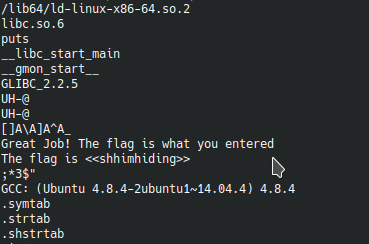
\includegraphics[width=7cm, height=5cm]{strings.png}
    \caption{Printable strings from challenge binary}
    \label{fig:my_label}
\end{figure}

\subsection{Ghidra SRE}

Ghidra Software Reverse Engineering\cite{ghidra} tool is a static analysis framework that provides analysis and views for a binary or firmware image. We will be using Ghidra to disassemble, and decompile the provided qualification binary and ultimately understand its functionality. 

\subsection{Firmware Exploitation}

Undefined behavior in a system that can be harnessed by an attacker is known as vulnerability. The usage of a vulnerability to induce anomalous behavior is what is known commonly as an exploit.  Firmware Exploitation is the act of exploiting vulnerabilities inside the firmware code, typically execute attacker-defined code, or bypass authentication. Stack based buffer overflows, use-after-frees, and return orient programming are common exploit techniques that can be used in firmware exploitation.

\subsection{Symbolic Execution}
During symbolic execution a program is analyzed at each stage. Symbolic values are used for variables at each stage, then upon reaching a desired state, a solver is used to solve those symbols for valued inputs which produce the desired results\cite{symmex}. One popular symbolic execution tool used later in this work is angr\cite{angr}.

\subsection{Fuzzing}

Fuzzing is a technique for discovering vulnerabilities in a system where test cases are created  which generates and provides mutated input to a system and monitors for exceptions. Fuzzing embedded targets can be made more difficult because those embedded devices require customized harnesses for providing that mutated input to device programs. Thus, many embedded targets require custom written fuzzers. However there are many publicly available fuzzers such as AFL\cite{afl}, and Radamsa\cite{radamsa} that work for general programs, and can be harnessed for embedded devices.

\subsection{RFID Security}
While RFID cards/chips can come in a variety of frequencies ranging from low frequency to ultra-high frequency, the devices tend to work in similar fashions. Historically these devices contain some string that is used for identification\cite{rfidsec2}, whether it be a person's ID card or a product in a store\cite{rfidsec2}.

Historically the largest threat to RFID based identification systems are spoofing and cloning of real identifications. Oftentimes this is done by being in close proximity of the target and using physical means for cloning IDs \cite{rfidsec1}.

As the field has progressed, there have been pushes to make the systems more complex, utilizing different cryptographic schemes to either block or increase the cost of historical attacks\cite{rfidsec1}\cite{rfidsec2}. While these do help with protecting against attacks, there is still the notable attack vector of dumped firmware. Even though it does not render the system insecure by itself, if an attacker is able to dump the firmware of an RFID receiver/scanner, they would be able to begin to test the firmware for vulnerabilities or logical flaws in code (for example flaws in cryptography algorithms) that might allow them to mount an attack against the system. 

\section{Qualification Binary}
\label{sec:attacks}

In this section we present approaches and solutions to the provided qualification binary. We start with a static analysis approach, then explore automated solutions, which could make solving complex binaries more feasible. 
\begin{figure}
    \centering
    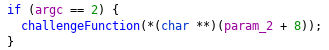
\includegraphics{argc.png}
    \caption{Decompiled functionality used to trigger the challengeFunction}
    \label{fig:my_label}
\end{figure}
\subsection{Static Analysis}
\subsubsection{Initial analysis and strings}
The goals during initial analysis are to obtain high level understandings of the qualifications executable characteristics such as architecture, exploit mitigations, and reactionary behavior when supplied with various forms of input. That input could be in the form of stdin, arguments, or input files, as an example.

Using file, the challenge binary is shown to be a 64-bit x86 binary. This binary contains several print-able strings, which are revealed using the strings command line utility, and are shown in Figure 1. Many of these strings are functions, section headers, and other garbage data. However, checking the printable strings revealed two possible flags: "Great Job! The flag is what you entered" and "The flag is shhimhiding". 

Knowing that the first flag is "shhimhiding" leaves the authors to find what triggers the former string.



Another command line utility "checksec" was used to see if there were any exploit mitigations present in the binary. The only protection reported was Data Execution Prevention, which allows for regions of memory to be specified as non-executable.

\subsubsection{Reverse engineering and the algorithm}
Using Ghidra to disassemble and decompile the executable, starting with the main function, it is shown that the program expects command line arguments to be given. The pointer to the first argument will then be passed over to the function "challengeFunction" as shown in Figure 2.


Decompiling the "challengeFunction" (Figure 3) will reveal to use the print statement that will give us the desired output of "Great Job! The flag is what you entered" along with some operations and "if statements" needed to be true to execute that print statement. The decompilation of the function is below with some retyping and changes to variable names to make cleaner. 

\begin{figure}
    \centering
    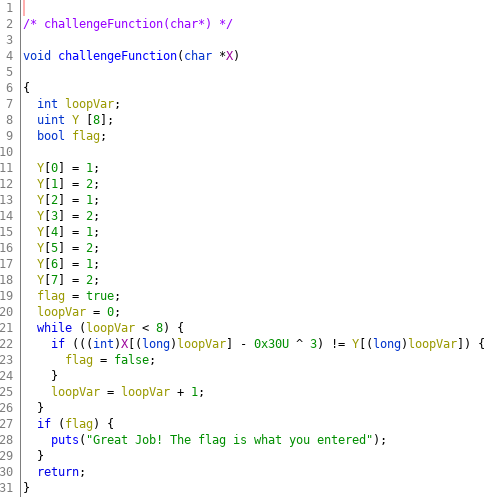
\includegraphics[width=8cm, height=8cm]{challenge.png}
    \caption{Decompiler output for challengeFunction}
    \label{fig:my_label}
\end{figure}

With the decompilation above, the first assignment we see is integers of 1's and 2's being assigned to an integer array \textit{Y}. Then, a while loop iterating though 8 characters of the command line argument. Operations are then performed on each byte, \textit{X}, and eventually compared to the value in the integer array according to the index of the loop variable. If after all the operations occur, and all of the results match with the value in the array \textit{Y}, according to index, we will have the "flag" variable left unchanged and the condition meet to print out the success string. The operations can be see on line 22 inside the if statement, and can be represented by the function below.
\begin{equation}
    f(x) = (x - 0x30) \oplus 3
\end{equation} 

\subsubsection{Solution}

With the information pulled from reverse engineering, its deduced that the program will take a single command line argument, iterating through the the first 8 characters, and subtracting each of them by 0x30 and xor'ing the result by 0x03. The final result of that, \textit{X}, will then be compared to an integer in the array [1, 2, 1, 2, 1, 2, 1, 2], \textit{Y}, according to its index (i.e \textit{X}[4] == \textit{Y}[4]). Using
\begin{equation}
    f(x) = (x - 0x30) \oplus 3
\end{equation} 
and the ASCII table to find the literal character '2' and '1' hold the numeric values of 0x32 and 0x31, which when used in the equation will result in the numeric 1's and 2's in the array. Providing the string "21212121" as the binary's first argument will result in the correct match for the values in the integer array, and the program outputting "Great Job! The flag is what you entered". 

\begin{figure}
    \centering
    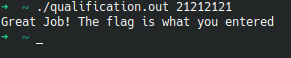
\includegraphics[width=6cm]{solution.png}
    \caption{Output from program when entering the second flag}
    \label{fig:my_label}
\end{figure}

\begin{figure}
    \centering
    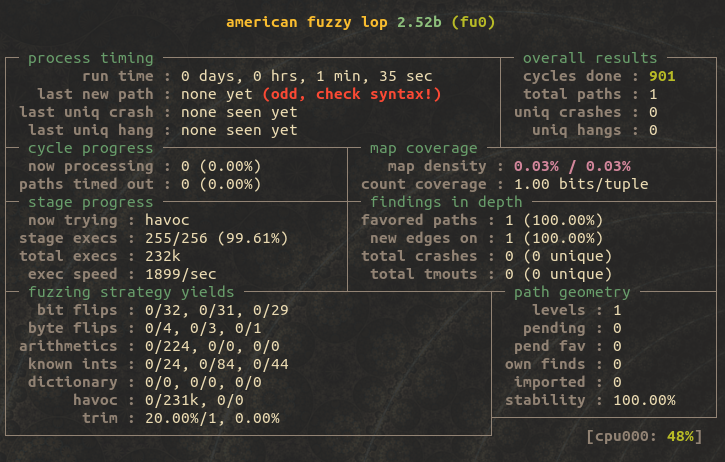
\includegraphics[width=6cm, height=4cm]{afl.png}
    \caption{Attempted AFL fuzzing, note the single total path}
    \label{fig:my_label}
\end{figure}

Thus the two flags recovered from static analysis of the challenge binary are a command line argument of "21212121" and the string "<<shhimhiding>>" from a secret function inside of the binary. 

\subsection{Automated Solutions}
While static analysis faired well for this challenge, more complex programs and algorithms might be solved more efficiently with automated solution. In this section we cover some approaches we took to attempt to solve the  challenge binary, with varying success.


\subsubsection{Symbolic Execution}
%make sure to note perf could/would likely be improved in this case via concolic execution, explian differences
For symbolic execution we used angr\cite{angr}. It is a python library which allows users to specify which features of a program to search for, then searches to execute the program in a way that satisfies those specifications. 

In our testing we assumed that the researcher who was looking to reverse engineer the program was able to the basic information from static analysis which includes the argument calls which trigger challengeFunction. 

From then we had angr find a suitable input that triggered an output containing the words 'flag' since we knew that we needed to trigger a print statement which included the word flag. The symbolic solution script then prints the input that led to that print. These files are attached to the hotcrp submission in .tar.gz form for artifact evaluation and future reproducability.

While running the solution script, assuming that the input was a string of integer values, it took only 16 seconds to reach the solution by itself. This time was measured on a Haswell processor manufactured in 2014. To simulate not knowing the keyspace of the input, the same solver was used with a keyspace of all printable bytes as input. That solution took 16.2 seconds, showcasing the strength of symbolic execution when working with larger keyspaces. While this may be relatively timely to develop and deploy when compared to looking at the decompiler output while doing static analysis, it is feasible that symbolic execution would help alleviate the necessary work for more complex algorithms, or larger programs.

\section{Finals Round Challenges}
During the finals round fives sets of challenges were released, with varying levels of difficulty. The authors took two approaches, each with different difficulties and achievement. These included symbolic execution with Angr, and static analysis with Ghidra.

\section{Angr in the Finals}
As a result of most of the challenges comprising of inputs that satisfy conditions within the binary, it was thought that Angr would suit these nicely, similarly to with the qualification binary.

The first difficulty when using Angr to automatically analyze and attempt to solve challenges was that the Cortex-M processor on the TeensyDuino uses Thumb2 code. Prior to manually setting angr to use this architecture Vex would generate invalid instructions and fail to decode some functions at all. 

After setting the correct architecture settings, Angr was able to traverse some challenge binary functions. The shortcoming with this approach was that it did not result in found paths, but rather each challenge that was traversed resulted in unconstrained variables, which are unsolvable by Angr. Thus, there were no finals round challenges solved using Angr.

\section{Static Analysis of Finals Challenges}
Static analysis was successfully used to solve a few of the finals round challenges. While stairs from challenge set A was a simple XORing problem, other challenges proved to be a bit more complex to decipher. Those challenges that were solved, their set, and related solution hashes are presented in section VI.

\section{Solved Finals Challenge Hashes}
In this section we present the challenges that the authors have solved, and the resulting challenge hashes.
\begin{table*}
\begin{center}
    \begin{tabular}{|c|c|c|}
        \hline
        challenge & set & hash\\
        \hline
        stairs & a & 396f4b1cdf1cc2e7680f2a8716a18c887cd489e12232e75b6810e9d5e91426c7 \\
        recess & c &  370815b8d8fde829f5c35f893d0b4139d61a775baa4181fcac1fffe014bde9ea \\
        break & c & 2d3448f09329f453e6f3a5403d89c061a9dabfbb9103ad6b8cc86d16345a7547 \\
        \hline
    \end{tabular}{}
\end{center}
\end{table*}


\section{Conclusion}
\label{sec:Concl}
In this paper we have presented the basics of reverse engineering and exploiting the firmware that provides functionality for RFID-based systems. Both manual static analysis and automated approaches such as symbolic execution and fuzzing were presented. All approaches were then used to attempt to solve the CSAW ESC 2019 qualification binary, with varying results explained. Both flags $"$21212121$"$ and "$<$$<$shhimhiding$>$$>$" were successfully recovered through those efforts. Static analysis was then used to solve multiple CSAW ESC finals round binaries. 


\begin{thebibliography}{00}
\bibitem{ghidra} National Security Agency ``Ghidra''. National Security Agency, 2019. https://ghidra-sre.org/

\bibitem{radamsa} Aki Helin ``Radamsa, a general-purpose fuzzer''. gitlab.com, 2019. https://gitlab.com/akihe/radamsa

\bibitem{afl} Michal Zalewski ``american fuzzy lop''. lcamtuf.coredump.cx, 2017. http://lcamtuf.coredump.cx/afl/

\bibitem{afl-argv} Michal Zalewski ``american fuzzy lop - sample argv fuzzing wrapper''. github.com, 2015. https://github.com/mirrorer/afl/blob/master/experimental/argv\_fuzzing/argv-fuzz-inl.h

% afl qemu blackbox
\bibitem{afl-qemu} Andrew Griffiths, Michal Zalewski ``   american fuzzy lop - high-performance binary-only instrumentation''. github.com, 2017. https://github.com/mirrorer/afl/blob/master/qemu\_mode/patches/afl-qemu-cpu-inl.h

\bibitem{angr} Shoshitaishvili, Yan and Wang, Ruoyu and Salls, Christopher and Stephens, Nick and Polino, Mario and Dutcher, Audrey and Grosen, John and Feng, Siji and Hauser, Christophe and Kruegel, Christopher and Vigna, Giovanni ``SoK: (State of) The Art of War: Offensive Techniques in Binary Analysis''. IEEE Symposium on Security and Privacy, 2016. 
%cite symex and concolicex 
\bibitem{symmex} James C. King ``Symbolic Execution and Program Testing''. Communications of the ACM, 1976. 

\bibitem{rfidsec1} Government of Hong Kong Special Administrative Region ``RFID SECURITY''. infosec.gov.hk, 2008. https://www.infosec.gov.hk/english/technical/files/rfid.pdf

\bibitem{rfidsec2} Francis Brown ``RFID Hacking Live Free or RFID Hard''. DEF CON 21, 2013. https://www.defcon.org/images/defcon-21/dc-21-presentations/Brown/DEFCON-21-Brown-RFID-Hacking-Updated.pdf
\end{thebibliography}
\vspace{12pt}
\end{document}
